\chapter{Практическая часть}

\section{Задание \No{}1}

Дана функция:
\begin{lstlisting}
(defun mystery (x)
    (list (second x) (first x))
)
\end{lstlisting}
Какие результаты вычисления следующих выражений?


\begin{lstlisting}
(mystery (one two))
\end{lstlisting}
\textbf{Результат:} ошибка - нет переменной ONE

\begin{lstlisting}
(mystery (last one two))
\end{lstlisting}
\textbf{Результат:} ошибка - нет переменной ONE

\begin{lstlisting}
(mystery free)
\end{lstlisting}
\textbf{Результат:} ошибка - нет переменной FREE

\begin{lstlisting}
(mystery (one 'two))
\end{lstlisting}
\textbf{Результат:} ошибка - нет переменной ONE

\section{Задание \No{}2}

Написать функцию, которая переводит температуру в системе Фаренгейта
температуру по Цельсию (defum f-to-c (temp) ...).

\begin{lstlisting}
;;; c = 5/9*(f-320)
(defun f-to-c (temp)
    (* (/ 5 9) (- temp 320))
)

(f-to-c 451) ;;; 655/9
\end{lstlisting}

\section{Задание \No{}3}

Что получится при вычисления каждого из выражений?

\begin{lstlisting}
(list 'cons t NIL)
\end{lstlisting}
\textbf{Результат:} (CONS T NIL)

\begin{lstlisting}
(eval (eval (list 'cons t NIL)))
\end{lstlisting}
\textbf{Результат:} ошибка - функция T не объявлена

\begin{lstlisting}
(apply #cons '(t NIL))
\end{lstlisting}
\textbf{Результат:} ошибка - неправильный формат комплексного числа

\begin{lstlisting}
(list 'eval NIL)
\end{lstlisting}
\textbf{Результат:} (EVAL NIL)

\begin{lstlisting}
(eval (list 'cons t NIL))
\end{lstlisting}
\textbf{Результат:} (T)

\begin{lstlisting}
(eval NIL)
\end{lstlisting}
\textbf{Результат:} NIL

\begin{lstlisting}
(eval (list 'eval NIL))
\end{lstlisting}
\textbf{Результат:}  NIL

\section{Задание \No{}4}

Написать функцию, вычисляющую катет по заданной гипотенузе и другому катету
прямоугольного треугольника, и составить диаграмму ее вычисления.

\begin{lstlisting}
(defun cathet (hypotenuse another)
    (sqrt (- (* hypotenuse hypotenuse) (* another another)))
)

(cathet 5 4) ;;; 3.0
\end{lstlisting}

Ниже представленна диаграмма вычисления данной программы.
\begin{figure}[H]
    \centering
    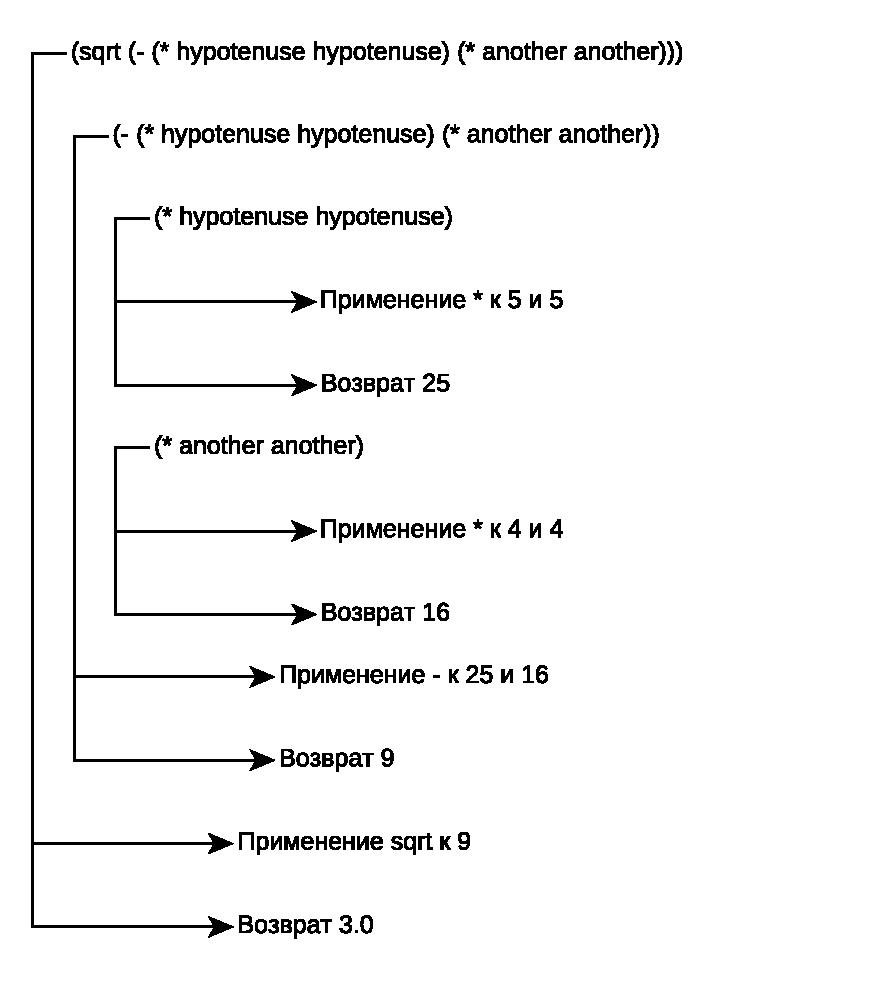
\includegraphics[scale=0.85]{data/pdf/task_1.pdf}
    \caption{Диаграмма задания 4}
\end{figure}

\section{Задание \No{}5}

Написать функцию, вычисляющую площадь трапеции по ее основаниям и
высоте, и составить диаграмму ее вычисления.

\begin{lstlisting}
(defun square (a b h)
    (* (/ (+ a b) 2) h)
)
(square 2 4 5) ;;; 15
\end{lstlisting}

Ниже представленна диаграмма вычисления данной функции.
\begin{figure}[H]
    \centering
    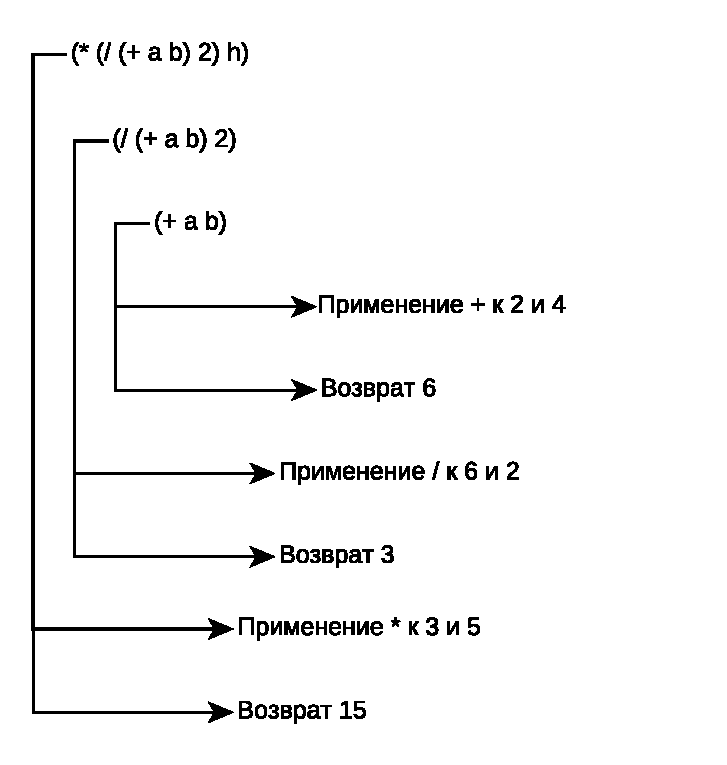
\includegraphics[scale=0.85]{data/pdf/task_2.pdf}
    \caption{Диаграмма задания 5}
\end{figure}
